\documentclass[conference]{IEEEtran}
\IEEEoverridecommandlockouts
% The preceding line is only needed to identify funding in the first footnote. If that is unneeded, please comment it out.
\usepackage{amsmath,amssymb,amsfonts,nccmath}
\usepackage{subfig}
\usepackage{svg}
\usepackage{graphicx}
\usepackage{algorithmic}
\usepackage{hyperref}
\usepackage{graphicx}
\usepackage{textcomp}
\usepackage{xcolor}
\usepackage{tabularx}
\usepackage[sorting=none,backend=biber,bibstyle=numeric,citestyle=numeric-comp]{biblatex}


\addbibresource{bibliography.bib}

\usepackage{quoting}
\quotingsetup{font=small, font=itshape}
\newcolumntype{P}[1]{>{\centering\arraybackslash}p{#1}}


\begin{document}

\title{HuggingGreen - A Probabilistic Attention-Based Method for Energy Efficiency}

\author{\IEEEauthorblockN{Mattia Limone}
\IEEEauthorblockA{\textit{Dipartimento di Informatica} \\
\textit{Università degli Studi di Salerno}}
\and
\IEEEauthorblockN{Carmine Iannotti}
\IEEEauthorblockA{\textit{Dipartimento di Informatica} \\
\textit{Università degli Studi di Salerno}}
}

\maketitle
\begin{abstract}
Vision Transformers (ViTs) have achieved state-of-the-art performance in many computer vision tasks. However, their high computational cost and energy consumption during training remain a major obstacle for their widespread adoption in resource-constrained scenarios. In this work, we propose a modified ViT architecture with probabilistic attention mechanisms that reduce the energy consumption during training without sacrificing the model's performance. Our approach utilize a probabilistic interpretation of the attention score in order to reduce the computational complexity required for self-attention, as well as a sparsity-inducing regularization term that encourages the attention weights to be more sparse. Additionally, we introduce a novel technique that selectively activates the attention mechanism only for important feature maps, further reducing energy consumption. We evaluate our proposed method on image classification and object detection task, and show that our method achieves comparable or better accuracy than the state-of-the-art ViT models while reducing energy consumption. The results aims to demonstrate the effectiveness of our modified ViT architecture in achieving energy-efficient training, which can benefit a wide range of applications, especially in resource-constrained environments. 

A PyTorch implementation can be found at: \href{https://github.com/MattiaLimone/HuggingGreen}{https://github.com/MattiaLimone/HuggingGreen}
\end{abstract}

\begin{IEEEkeywords}
ViT, Image Classification, Object Detection, Energy Consumption
\end{IEEEkeywords}

\section{Introduction}
For decades, image classification has been a prominent research area in computer vision. With the advancements in deep learning, models can now identify objects, patterns, and features in images with high accuracy, revolutionizing image recognition. Convolutional neural networks (CNNs) have been the dominant approach for image recognition tasks, including object detection, but recent research has shown that transformers can also achieve state-of-the-art performance in this domain. 

Transformers were initially developed for natural language processing tasks but have gained attention in the computer vision community due to their ability to model long-range dependencies and capture global context. The Vision Transformer (ViT) introduced by Dosovitskiy et al. \cite{DBLP:journals/corr/abs-2010-11929} has shown impressive performance in various image recognition tasks, surpassing the performance of CNNs on several benchmarks.

In this paper, we attempt to go further and study the energy impact of these architectures and propose a version of the same model that makes use of a probabilistic attention mechanism in order to reduce electricity consumption.

The paper is organized as follows. In Section \ref{relatedwork}, we provide an overview of related work on transformers and their applications in computer vision.  In Section \ref{goal}, we describe the work goal and the research questions this work is structured around. In Section \ref{dataset}, we will present the datasets that we will use as benchmarks to compare our model with others in literature. In Section \ref{executionplan}, we are going to describe the pipeline that we are going to follow. In Section \ref{metrics}, we are going to specify the evaluation metrics to compare the model with others. In Section \ref{architecture}, finally we will describe our architecture. In Section \ref{conclusion}, we will present the results of the experiment.

\begin{table}[h]
\centering
\begin{tabular}{|l|l|}
\hline
\textbf{Symbol} & \textbf{Description}        \\ \hline
$ \textbf{ViT}$              & Vision Transformer \\
$ \textbf{CNN}$              & Convolutional Neural Network \\
$ \textbf{RQs}$              & Research Question \\
$ \textbf{PDFs}$              & Probability Distribution Functions \\
$ \textbf{MLE}$              & Maximum Likelihood Estimation \\
$ \textbf{KWh}$              & KiloWatt-hour \\


\hline
\end{tabular}
\caption{Symbols used throughout the document}
\label{tab:symbols-table}
\end{table}

\section{Related works}
\label{relatedwork}
Convolutional neural networks (CNNs) have been widely used for image recognition tasks, but recent studies have shown that vision transformers (ViTs) can outperform CNNs on several benchmark datasets \cite{9790134}. However, ViTs have high computational and memory requirements, making them challenging to deploy on resource-constrained devices.



Transformers are a type of deep learning model that has revolutionized the field of natural language processing (NLP) and has also been used in computer vision and other fields.

Transformers were first introduced in 2017 by Vaswani et al.\cite{DBLP:journals/corr/VaswaniSPUJGKP17}. The key innovation of transformers is the use of self-attention mechanisms instead of recurrent neural networks (RNNs) or convolutional neural networks (CNNs), which were the predominant models for NLP at the time.

Self-attention is a mechanism that allows the model to weigh the importance of different parts of the input sequence when making predictions. This mechanism allows the model to handle long-range dependencies much better than RNNs or CNNs, which makes them ideal for NLP tasks such as language modeling, machine translation, and sentiment analysis.

Transformers consist of an encoder and a decoder. The encoder takes in the input sequence and produces a sequence of hidden representations, while the decoder takes in the output of the encoder and generates the output sequence. The key to the success of transformers is the use of multi-head attention, which allows the model to focus on different parts of the input sequence simultaneously.

Vision Transformer (ViT), introduced by Dosovitskiy et al.  \cite{DBLP:journals/corr/abs-2010-11929}, is a deep learning model that uses the transformer architecture for image classification. 

Traditionally, convolutional neural networks (CNNs) have been the dominant model architecture for image classification tasks. However, ViT uses the transformer architecture to process image data without using any convolutional layers.

In ViT, the image is divided into a set of fixed-size patches, and each patch is treated as a token. These tokens are then processed by a transformer encoder, which allows the model to capture global information about the image. The transformer encoder consists of multiple layers, each containing a multi-head self-attention mechanism and a position-wise feedforward network.

ViT achieves state-of-the-art results on several benchmark image classification datasets, including ImageNet and CIFAR-100. One of the benefits of ViT is that it allows for better generalization to out-of-distribution data since it relies on global features instead of local patterns.


To address the issues of energy efficiency, several techniques have been proposed to reduce the energy consumption of ViTs. One approach is to use algorithms or heuristics that delete the large amount of redundancy present in self-attention operations. 

For example Yangfan Li et al.\cite{li2022divit} propose a delta patch encoding which expresses information in a compressed, more space-efficient and communication-efficient manner and a novel algorithm design of differential attention that leverage this patch locality to avoid these redundancies without loss of accuracy. 

Instead Jing Liu et al. \cite{liu2022ecoformer} propose a new binarization paradigm customized to high-dimensional
softmax attention via kernelized hashing, called EcoFormer, to map the original queries and keys into low-dimensional binary codes in Hamming space. In this study based on PVTv2-B0 and
ImageNet-1K datasets EcoFormer achieves a 73\% reduction in on-chip energy footprint with only a slight performance drop of 0.33\% compared to the standard attention.

In addition, some studies instead have approached the problem of energy consumption in a different way, for example, Ibrahim et al. \cite{ibrahim2022imagesig} propose ImageSign, a methodology in which images are processed as signatures and processed through one-dimensional convolution (conv1d). Through this study, the authors were able to show that on some datasets they were able to drastically reduce both the number of parameters and the size of the model compared to a ViT, from 4,915,401 to 37,112 parameters and from 59.5 MB to 0.6 MB, respectively. In addition, they also managed to reduce the number of FLOPs from 4.65 to 1.69 without having a loss of accuracy; in fact, in one of their studies, permonances improved compared to ViTs, from 75.23\% to 95.02\%.

In 2021 Gabbur et al. \cite{DBLP:journals/corr/abs-2010-15583} proposed a probabilistic interpretation of attention and suggested the use of Expectation Maximization algorithms for online adaptation of key and value model parameters, which can improve transformer model performance in tasks that require adaptation to new information during inference. Based on this work we have implemented their solution in a ViT architecture to address if the solution can be used in offline learning and  Nguyen et al. \cite{DBLP:journals/corr/abs-2110-08678,} proposed a novel transformer architecture called Transformer-MGK, which replaces redundant attention heads in transformers with a mixture of Gaussian keys. Transformer-MGK accelerates training and inference, has fewer parameters, and achieves comparable or better accuracy across tasks than its conventional transformer counterpart. This work highlights the potential of using mixture models to improve transformer performance and reduce computational complexity.

Overall, these studies demonstrate the importance of addressing the energy efficiency of ViTs, and highlight several techniques that can be used to reduce their computational and memory requirements. Our work builds on these prior studies by proposing a new technique that combines pruning and knowledge distillation to improve the energy efficiency of ViTs while maintaining their accuracy.
\section{Goals and Research Questions}
\label{goal}
The goal of this study is to assess whether a probabilistic approach as well as different training techniques results in an energy-efficient model with less impact on the environment. Based on this, after an analysis on the topic, we have structured our research around three research questions (\textbf{RQs}).

\medskip

\fcolorbox{black}{blue!5!white}{

\begin{tabular}[t]{p{0.825\columnwidth}}
    \textbf{RQ$_{1}$.} \textit{Could a probabilistic approach lead to more energy efficient Transformer-based model?}
\end{tabular}
}

\medskip
\fcolorbox{black}{blue!5!white}{
\begin{tabular}[t]{p{0.825\columnwidth}}
    \textbf{RQ$_{2}$.} \textit{Does removing parts of the information based on a heuristic allow the model to converge sooner?}
\end{tabular}
}

\medskip
\fcolorbox{black}{blue!5!white}{
\begin{tabular}[t]{p{0.825\columnwidth}}
    \textbf{RQ$_{3}$.} \textit{Can different training techniques lead to lower energy consumption while preserving performance?}
\end{tabular}
}

\medskip

With the first research question (\textbf{RQ$_{1}$}), based on work of Movellan et al. \cite{DBLP:journals/corr/abs-2010-15583}, we want to show that it is possible to use the attention mechanism in a mixture model treating the keys and values as the data points to cluster, and the queries as the test points for which the probability density function is estimated. The attention weights can be used as the mixture weights, and the values associated with each key can be used as the component PDFs. The mixture model can be trained using the MLE method, with the attention mechanism serving as the mixture density estimator.

Through this described methodology, our goal is to test whether a probabilistic approach applied to a Transformer-based model is able to make it energy efficient. The results that will be given to us from these experiments will only be a baseline, and that is why \textbf{RQ$_{2}$} was introduced, so that we can test whether it is possible to optimize the energy efficiency not only at the training level, but also on the size of the input by going to eliminate part of the information using a heuristic. 

In particular, we will try to answer \textbf{RQ$_{2}$} by attempting to implement a feature selection layer that use an heuristic to select which part of the image pass to the Vision Transformer model. In a Vision Transformer architecture, each image is divided into $n$ patches. Given a threshold $k < n$ we are going to select the a $k$ sample of patches according to the probability distribution described by the contrast, variance or entropy value of the patches.

In particular, in order to validate our hypotheses, it is not possible to rely only on one instance of training because this is not enough. In fact, this is why (\textbf{RQ$_{3}$}) was introduced, in which we are going to test if different approaches of training in the Image Recognition task can lead to a faster training and thus lead to lower electricity consumption. In common practice, a transformer-based model first goes through a pre-training phase on a large amount of data and then is fine-tuned for the specific task. We are going to train the model in a different way hoping that it will need less time to achieve the same performance. Firstly a pre-training phase will be done but for much less epochs compared to the common practice, then the model will be trained using the hard-negative contrastive learning where the model is trained to distinguish between a positive pair (consisting of two samples that are similar or belong to the same class) and a hard-negative pair  (consisting of two samples that are dissimilar or belong to different classes) and only then will a specific fine-tuning phase be carried out.
\section{Dataset}
\label{dataset}
\begin{figure*}[!h]
  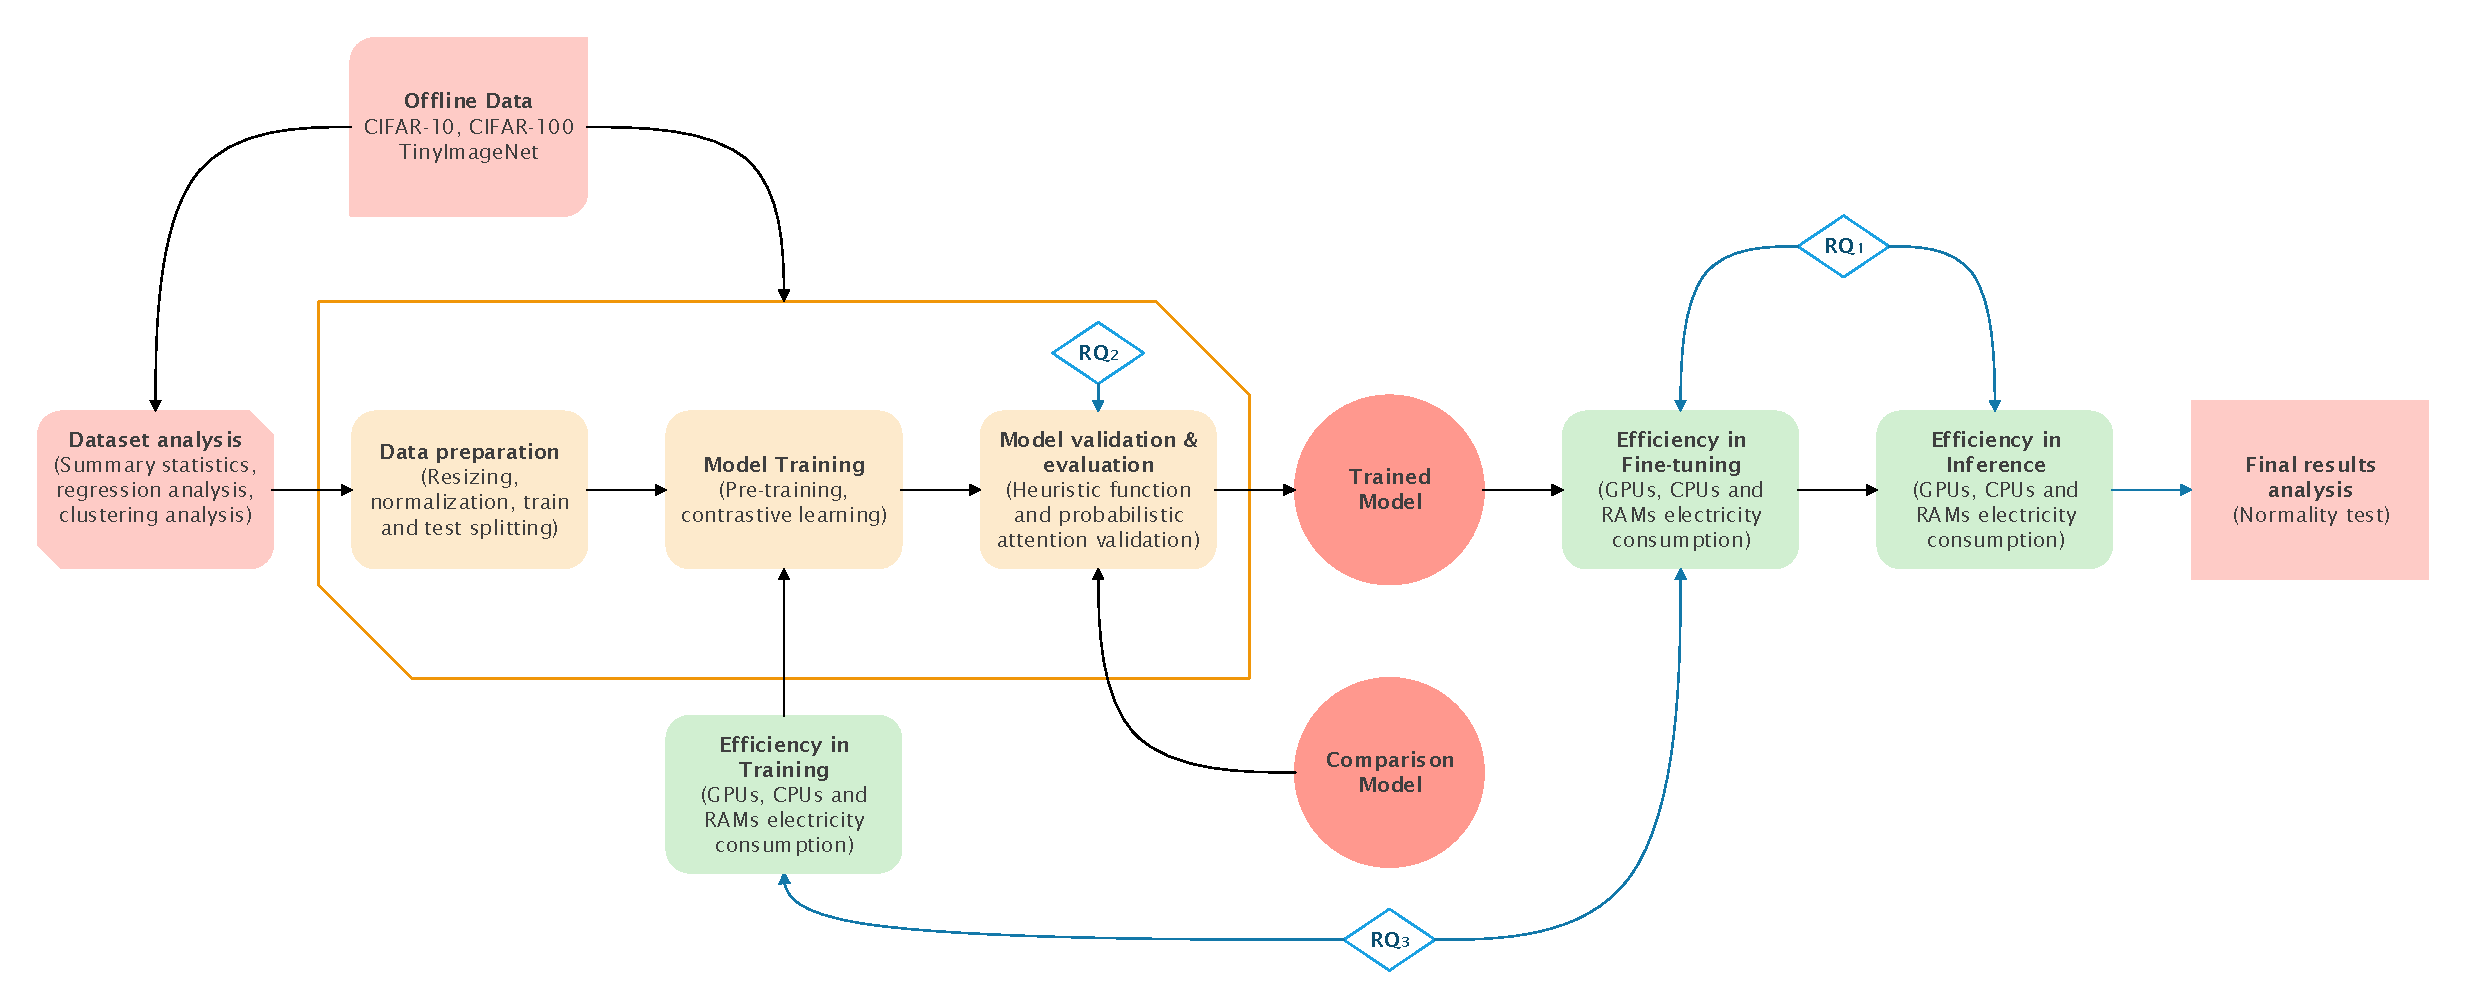
\includegraphics[width=\textwidth]{images/pipeline_final.pdf}
  \caption{Overview of the experiment pipeline}
  \label{pipeline}
\end{figure*}
The selection of a suitable dataset is a critical aspect of training machine learning models. The primary reason for choosing CIFAR-10/100 and TinynImageNet is the computational cost that larger datasets such as ImageNet and JFT-300M requires. These datasets contain a significantly larger number of images, and training on them requires a large amount of computational power and storage capacity. Given our research aim, which is to prove the energy efficiency of our modified Vit architecture, it is not feasible to use these datasets.

The datasets we have used are commonly used to train and evaluate machine learning models, particularly in the field of deep learning. Because the images are relatively small and low-resolution, the datasets can be trained on standard hardware without requiring a large amount of memory or computational resources. Additionally, because the images contain a wide variety of objects and backgrounds, they are a good benchmark for evaluating a model's ability to generalize to new, unseen data.

Over the years, many state-of-the-art models have been trained and evaluated on these datasets, including various convolutional neural network (CNN) and Vision Transformer (ViT) architectures. Achieving high accuracy on these datasets has become a standard benchmark for evaluating the performance of image classification models.

This decision allows us to focus on proving the energy efficiency of our architecture, which is the primary objective of our research.
CIFAR-10, CIFAR-100 are benchmark datasets commonly used for image classification tasks in computer vision research while Tiny ImageNet can give us a good understanding on the generalization capacity of the model. 

CIFAR-10 consists of 60,000 32x32 color images in 10 classes, with 6,000 images per class. The 10 classes are: airplane, automobile, bird, cat, deer, dog, frog, horse, ship, and truck.

CIFAR-100 also consists of 60,000 32x32 color images but divided in 100 classes, with 600 images per class. The 100 classes are grouped into 20 superclasses, each containing 5 subclasses. For example, the "aquatic mammals" superclass contains the "beaver", "dolphin", "otter", "seal", and "whale" subclasses.

Tiny ImageNet is a reduced version of the ImageNet dataset, which is a large-scale image dataset used for training deep learning models for computer vision tasks. The Tiny ImageNet dataset consists of 200 classes, each with 500 training images and 50 validation and test images. The images in this dataset are of size 64x64 pixels, significantly smaller than the images in the original ImageNet dataset.


\section{Execution Plan}
\label{executionplan}

The general execution pipeline, in figure \ref{pipeline}, provides an overview of the steps that have been followed. Hereafter, we will analyse for each research question how the experiment was conducted.
\subsection{\textbf{RQ$_{1}$} - Comparing a standard ViT with Our Proposal} 
After implementing in PyTorch our architecture described in  section \ref{architecture} we are going to train from scratch a ViT and our model and comparing them using the metrics explained in section \ref{metrics}.
For the energy efficiency analysis we will use CodeCarbon, which provides an accurate estimation of the energy producted by RAM, GPUs and CPUs during the executing of the code (we will use Colab to perform the operations in as isolated an environment as possible \textit{"Intel Xeon @ 2.20GHz and Tesla T4 GPU"}). 

We will perform a statistical validity test with null hypothesis stating that the sample (Electric energy consumed repeating the same experiment) follows a normal PDF and alternative hypothesis stating that it does not come from that distribution:
\begin{itemize}
    \item We will perform the Shapiro-Wilk test with significance level 0.05 in the hope of validating the null hypothesis 
    \item If the tests confirm the null hypothesis, then the energy values we will report will be the average of the calculated values.
    \item Finally, we will calculate the Carbon Intensity, which is the grams of CO$_2$ produced by running the code as the product of the Net Carbon Intensity (A weighted average of the emissions from the different energy sources that are used to generate electricity consumed by the Cloud provider or Country) and the KWh consumed.
\end{itemize}

\subsection{\textbf{RQ$_{2}$} - In Search of Heuristic that lead to a faster convergence}
When a human being is asked to understand an object represented on an image, a logical process is generally carried out that leads to discarding all information that does not concern the object itself. Based on this theory, we will implement a feature selection layer based on three different heuristics.
Given that every patch in which the image is divided is an $n \times n$ matrix the value of each patch $x$ is calculated as follows:
\begin{itemize}
    \item Contrast (Figure \ref{fig:dog_contrast}):  $$F(x) =  \frac{max(x) - min(x) + 10^{-8}}{max(x) + min(x)}$$ 
   
    \item Variance (Figure \ref{fig:dog_variance}): $$F(x) =  \frac{\sum_{i=1}^n\left(x_i-\overline{\mathbf{x}}\right)^2}{n-1}$$
       
    \item Entropy (Figure \ref{fig:dog_entropy}): $$F(x) =  -\sum_{i=1}^{n}(p_i * log2(p_i))$$\\ where $$p_i = \frac{count(i)}{N}$$
        
\end{itemize}
    \begin{figure}[!htp]
        \centering
        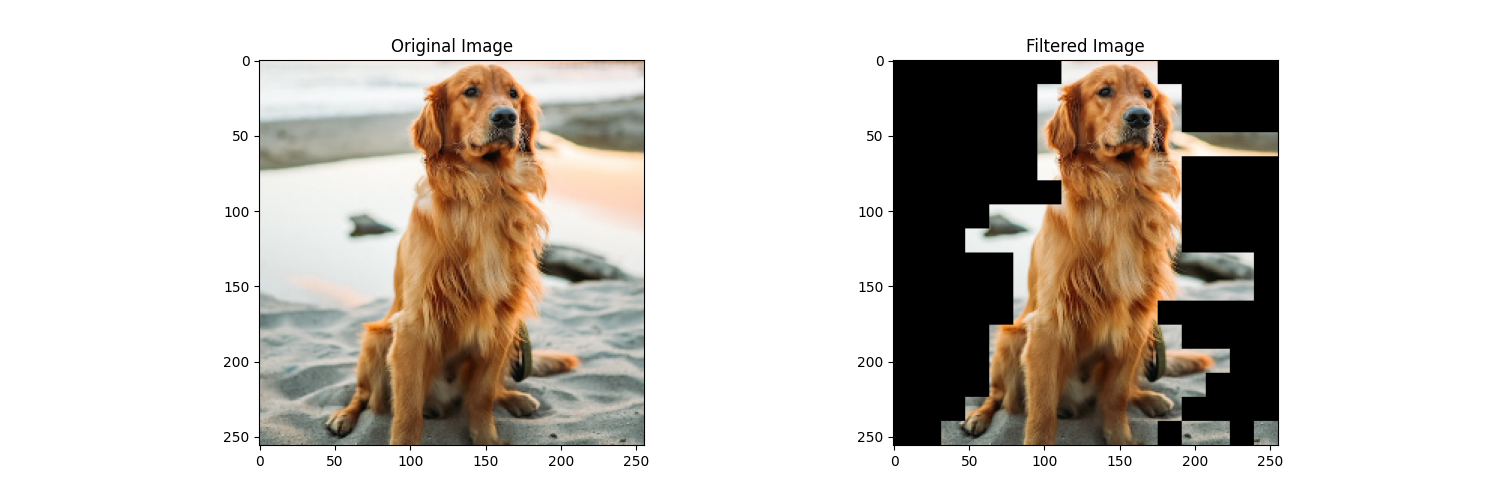
\includegraphics[width=\columnwidth]{images/dog_contrast.png}
        \caption{Image filtered based on contrast values distribution preserving 50\% of image}
        \label{fig:dog_contrast}
    \end{figure}
     \begin{figure}[!htp]
        \centering
        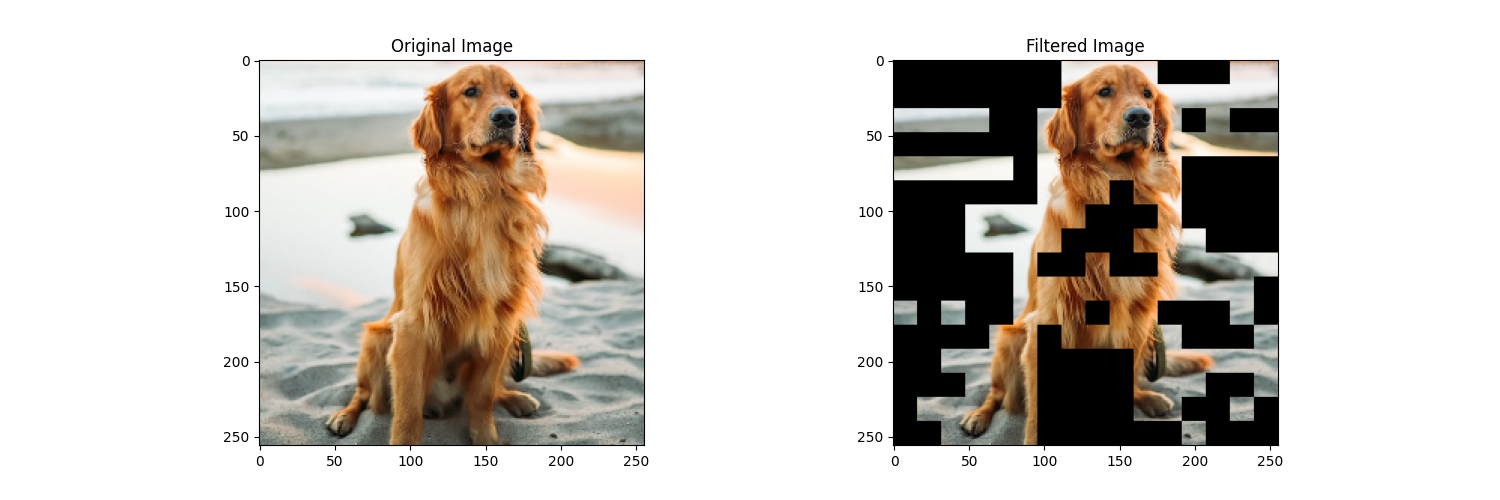
\includegraphics[width=\columnwidth]{images/dog_variance.png}
        \caption{Image filtered based on variance values distribution preserving 50\% of image}
        \label{fig:dog_variance}
    \end{figure}
    \begin{figure}[!htp]
        \centering
        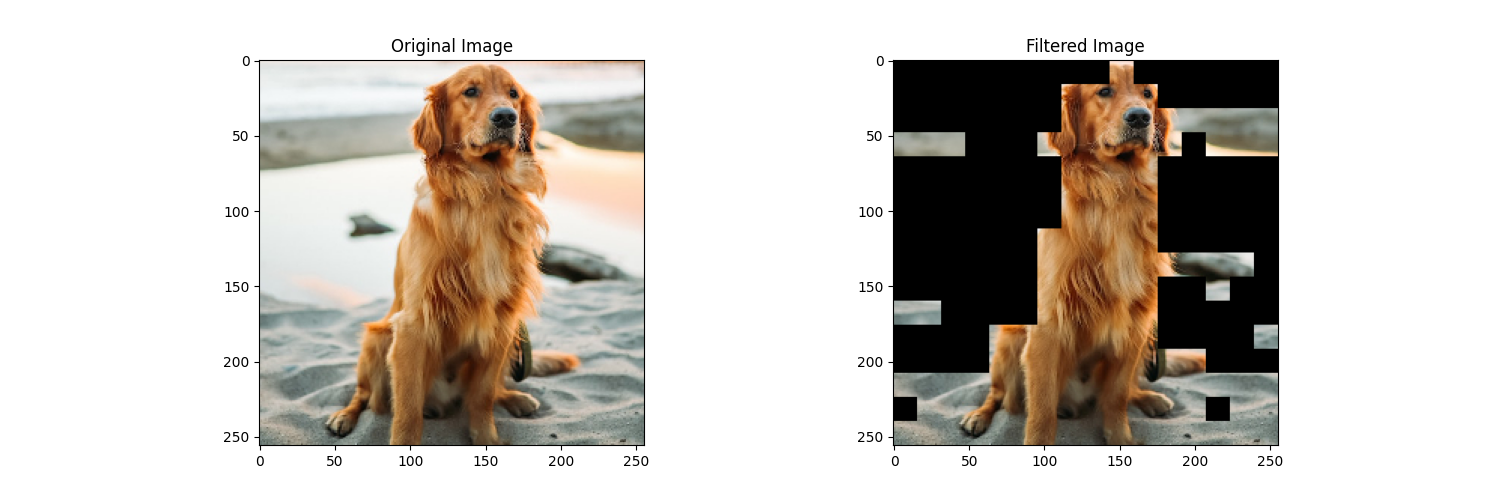
\includegraphics[width=\columnwidth]{images/dog_entropy.png}
        \caption{Image filtered based on contrast entropy distribution preserving 50\% of image}
        \label{fig:dog_entropy}
    \end{figure}
\subsection{\textbf{RQ$_{3}$} - Assessing the Performance of Our Model on different training technique} In this phase we will train our model using two different techniques

1) Pre-training + Fine-tuning

2) Pre-training + Contrastive Learning + Fine-tuning
\\
Each phase will be executed as follows:
\begin{itemize}
    \item Pre-training: the model will be trained on a large amount of unlabeled data to learn general features. In our pre-training, the model is trained on ImageNet using a self-supervised task called 'masked language modeling.' This involves randomly masking some patches of the input image and then training the model to predict the masked patches. This way, the model learns to represent the image in terms of meaningful patches of varying sizes and positions.

    \item Contrastive Learning: after pre-training, the model will be further fine-tuned using contrastive learning, which is a form of self-supervised learning. In contrastive learning, the model learns to distinguish between similar and dissimilar image patches by projecting them into a high-dimensional space and comparing their distances. This way, the model learns to identify patterns and features that are relevant for the downstream task, such as image recognition.

    \item Fine-tuning: once the model has been pre-trained and fine-tuned with contrastive learning, it will be further fine-tuned onimage recognition task on CIFAR-10/CIFAR-100. During fine-tuning, the model is trained on labeled data with a supervised learning approach. In this phase, the last few layers of the model are replaced with new ones, and only the newly added layers are trained on the specific task, while the earlier layers are frozen to retain the learned features. This way, the model can adapt to the specific dataset and learn to recognize the relevant features for the task at hand.
\end{itemize}
\section{Evaluation Metrics}
\label{metrics}
Since the goal of our work is to obtain a more energy-efficient model, the energy consumption due to the use of RAMs, GPUs and CPUs will be monitored throughout the pipeline in order to identify the most affected hardware parts.

Furthermore, since we aimed to build a model that has comparable performance to other proposals in the literature, the trade-off between Energy Consumption/micro-average F1 Score (\ref{eq:3}) will also be considered.

The micro-average F1 score (\ref{eq:3}) is a commonly used performance metric in machine learning classification tasks. It is a type of F1 score that is calculated by taking the overall precision and recall across all classes, and then using these values to compute a single F1 score.

In order to calculate the micro-average F1 score, we first need to calculate the precision and recall for each class separately. Precision (\ref{eq:1}) measures the fraction of true positives out of all predicted positives for a given class, while Recall (\ref{eq:2}) measures the fraction of true positives out of all actual positives for that class.

Once we have calculated the precision and recall for each class, we can compute the micro-average F1 score as the harmonic mean of the overall precision and recall:

\begin{equation} \label{eq:1}
Precision_{\mu\text{-}avg} = \frac{\sum_{i=1}^{n} TP_{i}}{\sum_{i=1}^{n} TP_{i} + \sum_{i=1}^{n} FP_{i}}
\end{equation}
\begin{equation} \label{eq:2}
Recall_{\mu\text{-}avg} = \frac{\sum_{i=1}^{n} TP_{i}}{\sum_{i=1}^{n} TP_{i} + \sum_{i=1}^{n} FN_{i}}\\
\end{equation}
\begin{equation} \label{eq:3}
F1\;Score_{\mu\text{-}avg} = 2 \cdot \frac{Precision_{\mu\text{-}avg} \cdot Recall_{\mu\text{-}avg}}{Precision_{\mu\text{-}avg} + Recall_{\mu\text{-}avg}}
\end{equation}
\section{Architecture}
\label{architecture}
Our ViT Architecture in Figure \ref{fig:ViTArchi} follows a three-stage process to process an input image:
\begin{itemize}
    \item Patch Selection: The input image is divided into a grid of fixed-size non-overlapping patches, typically 16x16 pixels in size. For each patch is calculated a score based on an heuristic (contrast/variance/entropy). The calculated values are interpreted as a probability distribution and a $k$ sample of patches is selected and passed to next step. The number of patches is determined by the size of the input image and the patch size.
    \item Patch Embeddings:  Each patch is then linearly projected to a low-dimensional space to obtain a patch embedding vector. The patch embeddings are arranged in a sequence to form the input to the transformer encoder. 
    \item Transformer Encoder: The patch embeddings are fed into a modified transformer encoder, which consists of multiple identical layers of self-attention and feed-forward layers. The self-attention mechanism allows the model to attend to different parts of the image and model the spatial relationships between patches. The feed-forward layers process the information from the previous layers and output a sequence of feature vectors.
\end{itemize}


    \begin{figure}[htp]
        \centering
        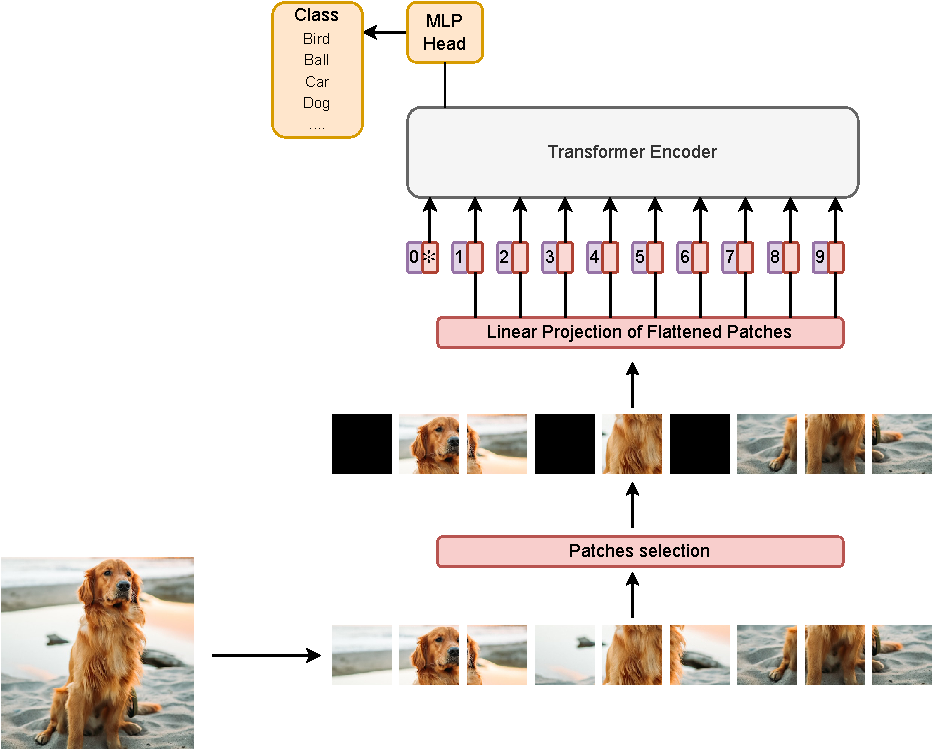
\includegraphics[height=7cm]{images/Vision Transformer Diagram.drawio.pdf}
        \caption{Our ViT Architecture}
        \label{fig:ViTArchi}
    \end{figure}


In this particular implementation, figure \ref{fig:TransformereNCODER}, of the Transformer Encoder block, the Multi-Head Attention layer has been modified to be probabilistic in nature. Specifically, the attention weights computed by the layer are used as mixture weights and the values associated with each key are used as the component of the PDFs.

This modification allows for a more flexible and expressive representation of the attention mechanism. By using a probabilistic approach, the model can capture a wider range of dependencies between different positions in the sequence.
    \begin{figure}[htp]
        \centering
        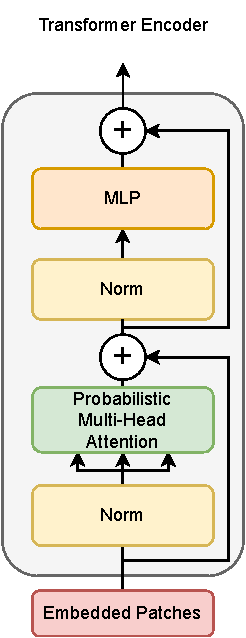
\includegraphics[height=7cm]{images/Transformer Encoder.drawio.pdf}
        \caption{Modified Transformer Encoder Block}
        \label{fig:TransformereNCODER}
    \end{figure}

\section{Conclusion}
\label{conclusion}
Experiment not yet performed
\section{Future plans}
\label{future}
In this paper, we presented HuggingGreen, a probabilistic attention-based method with the aim of reducing the environmental impact of transformer-based neural network models. However, there are several avenues for future research that could build upon our work and further advance the field of energy-efficient machine learning.

One potential direction for future research is to investigate the effectiveness of HuggingGreen on larger and more complex datasets. Probably it is possible that the performance of our method may degrade when faced with larger datasets or datasets with more different input features. Therefore, future research could focus on developing modifications to HuggingGreen that enable it to scale to larger datasets without sacrificing performance.

Another area for future investigation is the potential for incorporating HuggingGreen into existing deep learning architectures (e.g. ResNet50, EfficientNetV2).

Finally, future research could explore the application of HuggingGreen to real-world energy-efficient machine learning problems because it is important to validate our method on real-world sceniario to ensure its practical effectiveness. In particular, future research could focus on the deploy phase of an HuggingGreen-based model.

In summary, we hope that our work on HuggingGreen provides a foundation for future research on energy-efficient machine learning. We believe that the potential for further improvements and applications of this method is vast, and we look forward to seeing how the field of energy-efficient machine learning continues to evolve in the coming years.
\printbibliography[heading=bibintoc]
\end{document}